\chapter{Mechanical Design and \\Integration}

\section{Enclosure Overview}
The system is housed within a compact, custom-designed two-part enclosure. It should be noted that this mechanical design represents the \textit{external monitor configuration} of the system, tailored specifically for its use as a standalone, inline diagnostic tool. For future deployments where the measurement and communication circuitry are integrated directly into the internal architecture of a commercial power bank, the external case will no longer apply. In such integrated configurations, the final enclosure and physical constraints will be defined entirely by the customer (the power bank manufacturer) to align with their specific industrial design.

\subsection{Assembly Components}
The physical construction of the device is achieved through a multi-part mechanical assembly. The complete system comprises the custom two-part plastic enclosure (top and bottom covers), a dedicated clear screen cover to protect the display, the fully populated Printed Circuit Board (PCB), and the required mounting hardware. Table~\ref{tab:mech_components} details each of these individual physical components as illustrated in the exploded view of the system (Figure~\ref{fig:mech_exploded}).

\begin{figure}[H]
    \centering
    % Update the filename/path if necessary
    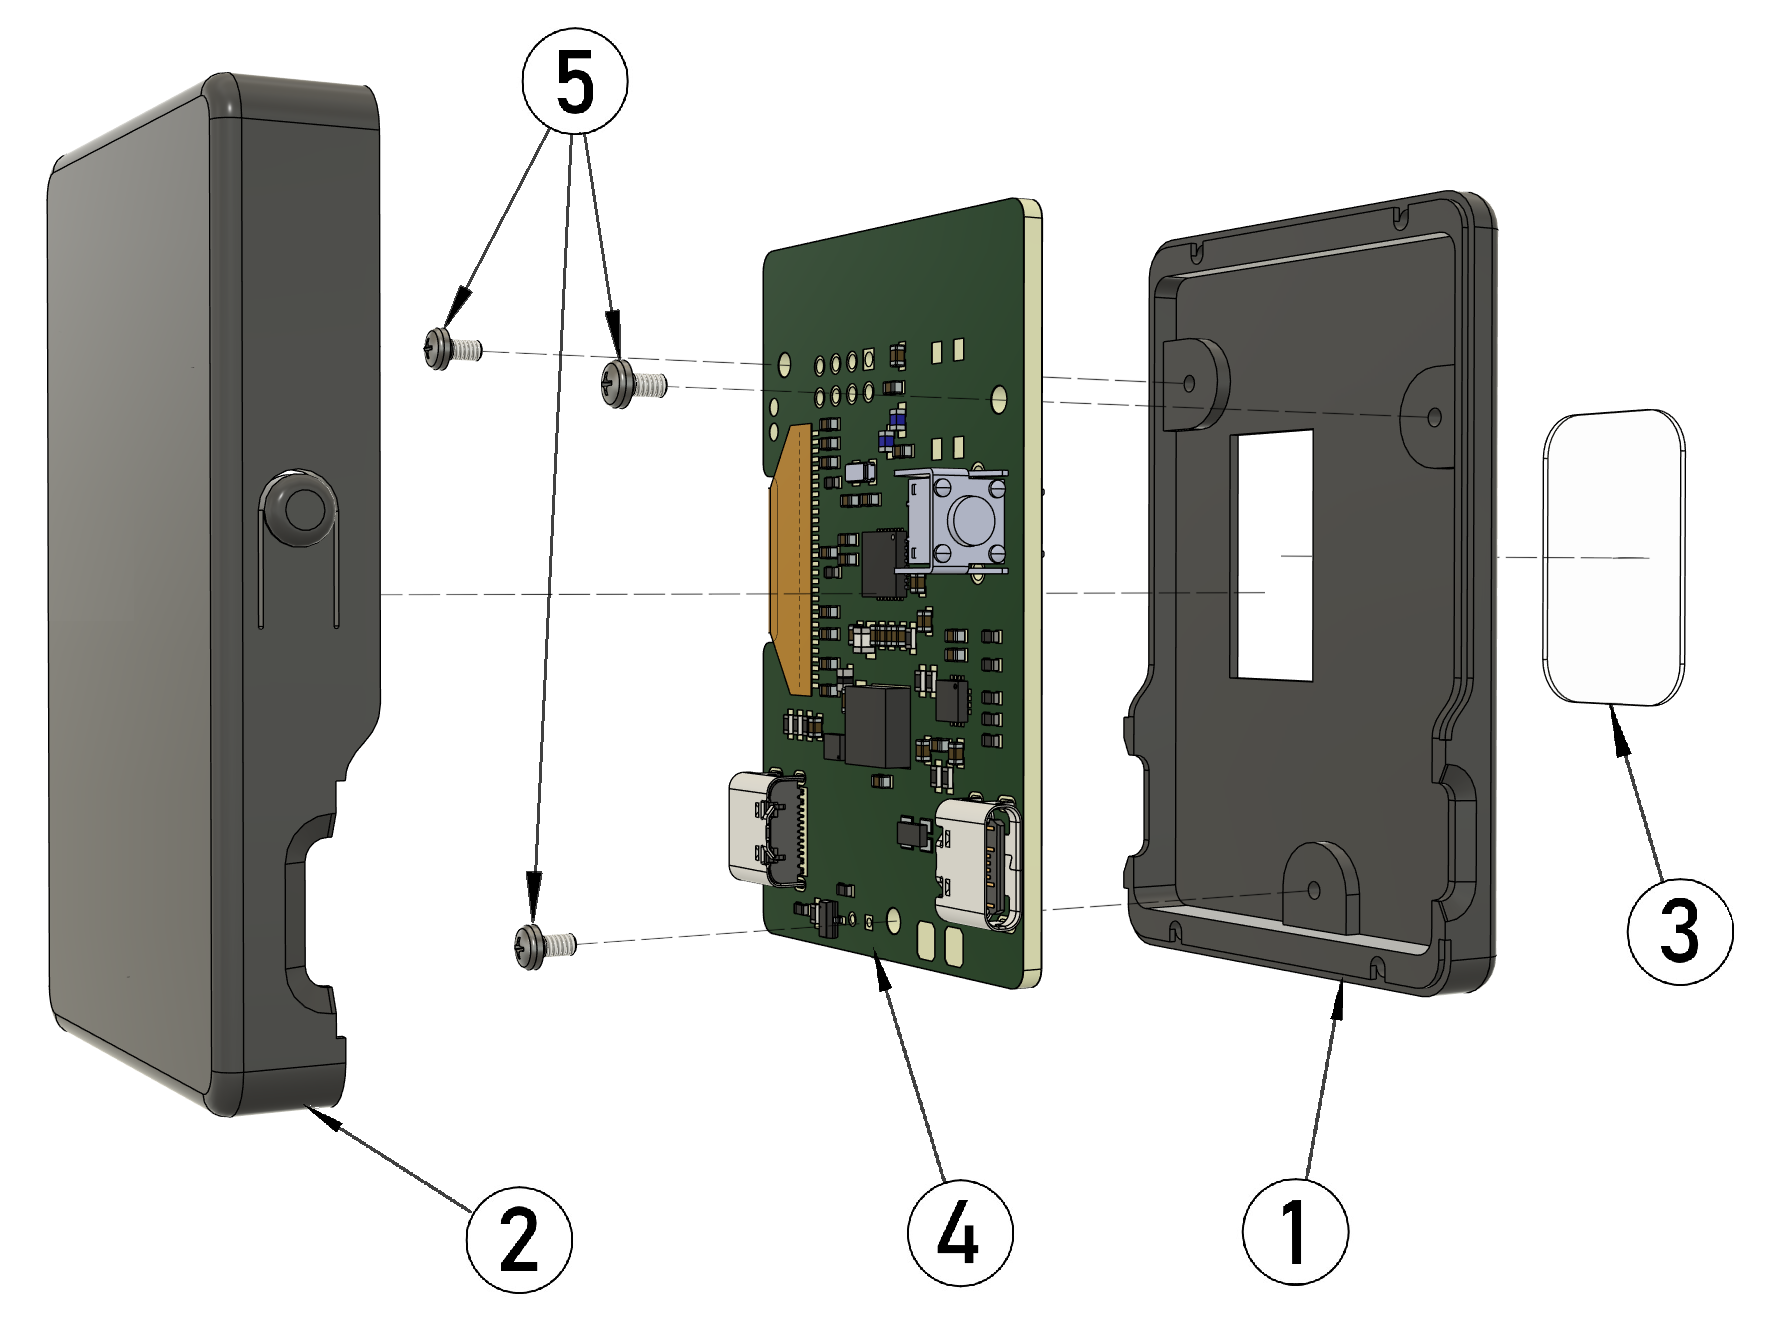
\includegraphics[width=0.9\textwidth]{figures/mech_assembly.png}
    \caption{Exploded 3D view of the system's mechanical assembly.}
    \label{fig:mech_exploded}
\end{figure}

\begin{table}[H]
    \centering
    \renewcommand{\arraystretch}{1.4}
    \caption{Description of the primary mechanical assembly components.}
    \label{tab:mech_components}
    
    \begin{tabularx}{\textwidth}{|c|l|X|}
    \hline
    \textbf{No.} & \textbf{Name} & \textbf{Description} \\
    \hline
    
    \textbf{1} & Top Cover & Upper half of the protective enclosure. \\
    \hline
    
    \textbf{2} & Bottom Cover & Bottom half of the protective enclosure. \\
    \hline

    \textbf{3} & Screen Cover & Clear cover for the device display. \\
    \hline

    \textbf{4} & PCB & The production version of the 4-layer Printed Circuit Board.. \\
    \hline

    \textbf{5} & Mounting Screws & Three M1.6 x 3 screws used to secure the pcb on the top cover \\
    \hline        
    
\end{tabularx}
\end{table}


\subsection{External Interfaces and Connectivity}

Figure~\ref{fig:mech_interface} illustrates the fully assembled device, with its primary external interfaces and ports detailed in Table~\ref{tab:user_interface}.


\begin{figure}[H]
    \centering
    % Update the filename/path if necessary
    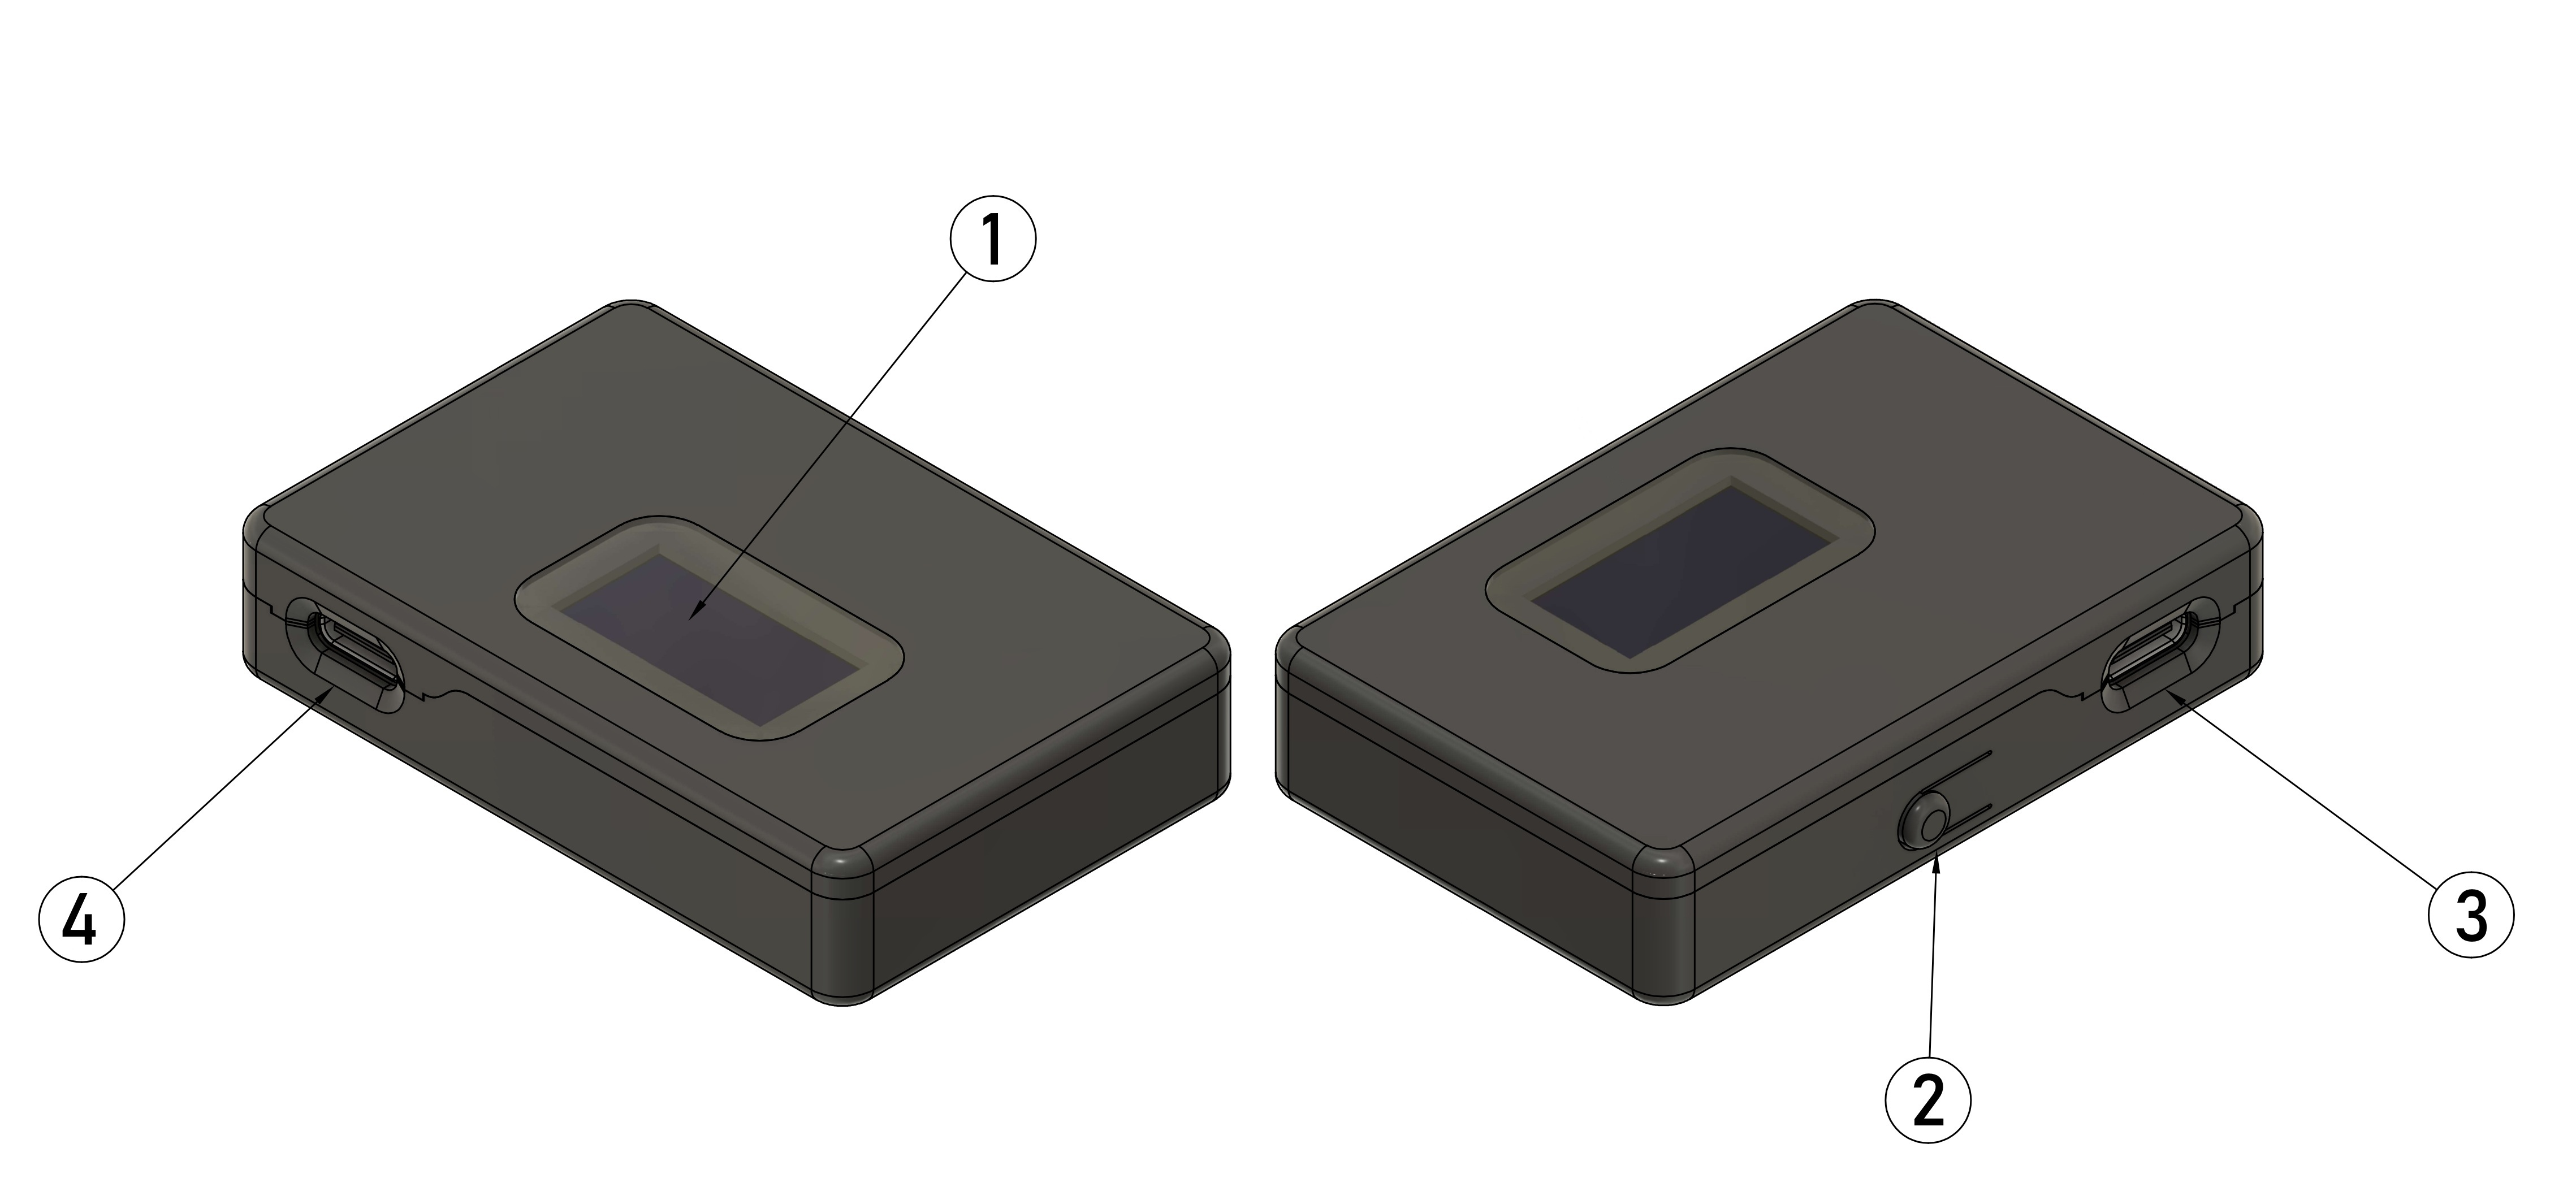
\includegraphics[width=\textwidth]{figures/mech_components.jpg}
    \caption{External view of the fully assembled system highlighting the key user interfaces and connectivity.}
    \label{fig:mech_interface}
\end{figure}


\begin{table}[H]
    \centering
    \renewcommand{\arraystretch}{1.4}
    \caption{Description of the external interfaces.}
    \label{tab:user_interface}
    
    \begin{tabularx}{\textwidth}{|c|l|X|}
        \hline
        \textbf{No.} & \textbf{Name} & \textbf{Description} \\
        \hline

        \textbf{1} & Display & Device display accessible through the enclosure cutout. \\
        \hline

        \textbf{2} & Button Actuator & User button actuator directly embedded in the protective enclosure. \\
        \hline

        \textbf{3} & Input Port & Power port connected to the powerbank or power source. \\
        \hline

        \textbf{4} & Output Port & Power port connected to the loaded device or battery charger. \\
        \hline
        
    \end{tabularx}
\end{table}